% This file is generated by the MATLAB m-file laprint.m. It can be included
% into LaTeX documents using the packages graphicx, color and psfrag.
% It is accompanied by a postscript file. A sample LaTeX file is:
%    \documentclass{article}\usepackage{graphicx,color,psfrag}
%    \begin{document}% This file is generated by the MATLAB m-file laprint.m. It can be included
% into LaTeX documents using the packages graphicx, color and psfrag.
% It is accompanied by a postscript file. A sample LaTeX file is:
%    \documentclass{article}\usepackage{graphicx,color,psfrag}
%    \begin{document}% This file is generated by the MATLAB m-file laprint.m. It can be included
% into LaTeX documents using the packages graphicx, color and psfrag.
% It is accompanied by a postscript file. A sample LaTeX file is:
%    \documentclass{article}\usepackage{graphicx,color,psfrag}
%    \begin{document}% This file is generated by the MATLAB m-file laprint.m. It can be included
% into LaTeX documents using the packages graphicx, color and psfrag.
% It is accompanied by a postscript file. A sample LaTeX file is:
%    \documentclass{article}\usepackage{graphicx,color,psfrag}
%    \begin{document}\input{ETT}\end{document}
% See http://www.mathworks.de/matlabcentral/fileexchange/loadFile.do?objectId=4638
% for recent versions of laprint.m.
%
% created by:           LaPrint version 3.16 (13.9.2004)
% created on:           23-Mar-2016 13:43:56
% eps bounding box:     16 cm x 12 cm
% comment:              
%
%\begin{psfrags}%
%\psfragscanon%
%
% text strings:
\psfrag{s06}[t][t]{\fontsize{8}{12}\fontseries{m}\mathversion{normal}\fontshape{n}\selectfont \color[rgb]{0,0,0}\setlength{\tabcolsep}{0pt}\begin{tabular}{c}$\test = [\SI{}{ms}]$\end{tabular}}%
\psfrag{s07}[b][b]{\fontsize{8}{12}\fontseries{m}\mathversion{normal}\fontshape{n}\selectfont \color[rgb]{0,0,0}\setlength{\tabcolsep}{0pt}\begin{tabular}{c}$\e{\ers}{\ers}  = [\SI{}{bits/s/Hz}]$\end{tabular}}%
\psfrag{s11}[][]{\fontsize{10}{15}\fontseries{m}\mathversion{normal}\fontshape{n}\selectfont \color[rgb]{0,0,0}\setlength{\tabcolsep}{0pt}\begin{tabular}{c} \end{tabular}}%
\psfrag{s12}[][]{\fontsize{10}{15}\fontseries{m}\mathversion{normal}\fontshape{n}\selectfont \color[rgb]{0,0,0}\setlength{\tabcolsep}{0pt}\begin{tabular}{c} \end{tabular}}%
\psfrag{s14}[t][t]{\fontsize{8}{12}\fontseries{m}\mathversion{normal}\fontshape{n}\selectfont \color[rgb]{0,0,0}\setlength{\tabcolsep}{0pt}\begin{tabular}{c}$\pco$\end{tabular}}%
\psfrag{s18}[l][l]{\fontsize{8}{12}\fontseries{m}\mathversion{normal}\fontshape{n}\selectfont \color[rgb]{0,0,0}Empirical}%
\psfrag{s19}[l][l]{\fontsize{8}{12}\fontseries{m}\mathversion{normal}\fontshape{n}\selectfont \color[rgb]{0,0,0}$\e{\ers}{\ers}$]}%
\psfrag{s20}[l][l]{\fontsize{8}{12}\fontseries{m}\mathversion{normal}\fontshape{n}\selectfont \color[rgb]{0,0,0}$\pco$}%
\psfrag{s21}[l][l]{\fontsize{8}{12}\fontseries{m}\mathversion{normal}\fontshape{n}\selectfont \color[rgb]{0,0,0}Empirical}%
%
% axes font properties:
\fontsize{8}{12}\fontseries{m}\mathversion{normal}%
\fontshape{n}\selectfont%
%
% xticklabels:
\psfrag{x01}[t][t]{0}%
\psfrag{x02}[t][t]{0.5}%
\psfrag{x03}[t][t]{1}%
\psfrag{x04}[t][t]{1.5}%
\psfrag{x05}[t][t]{2}%
\psfrag{x06}[t][t]{2.5}%
\psfrag{x07}[t][t]{0}%
\psfrag{x08}[t][t]{0.5}%
\psfrag{x09}[t][t]{1}%
\psfrag{x10}[t][t]{1.5}%
\psfrag{x11}[t][t]{2}%
\psfrag{x12}[t][t]{2.5}%
%
% yticklabels:
\psfrag{v01}[l][l]{0.50}%
\psfrag{v02}[l][l]{0.60}%
\psfrag{v03}[l][l]{0.70}%
\psfrag{v04}[l][l]{0.80}%
\psfrag{v05}[l][l]{0.90}%
\psfrag{v06}[l][l]{1.00}%
\psfrag{v07}[l][l]{}%
\psfrag{v08}[r][r]{6.89}%
\psfrag{v09}[r][r]{6.93}%
\psfrag{v10}[r][r]{6.96}%
\psfrag{v11}[r][r]{7.00}%
\psfrag{v12}[r][r]{7.04}%
\psfrag{v13}[r][r]{7.07}%
\psfrag{v14}[r][r]{}%
%
% Figure:
%\resizebox{8cm}{!}{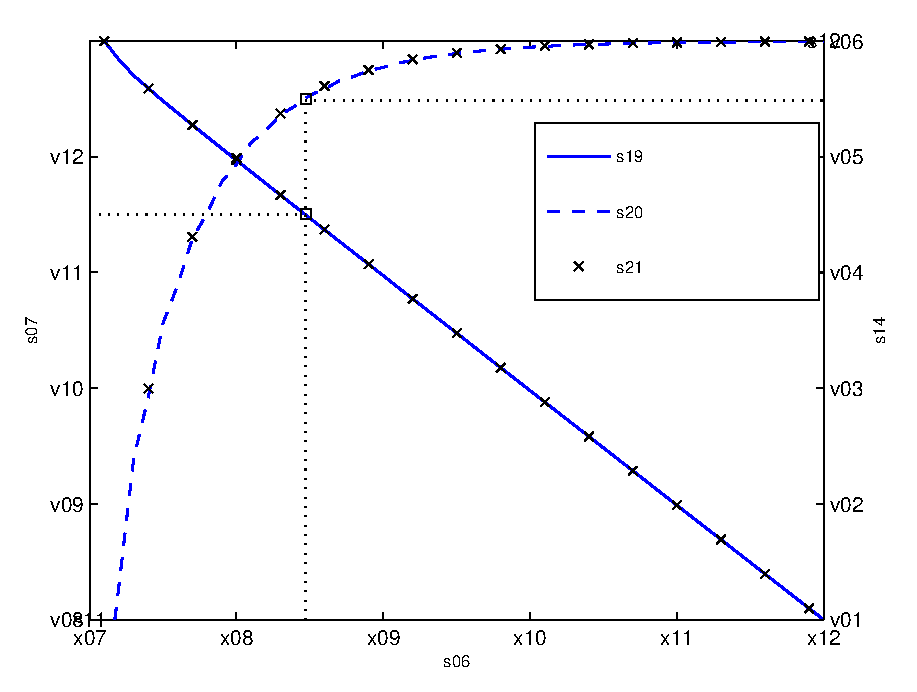
\includegraphics{ETT.eps}}%
%\end{psfrags}%
%
% End ETT.tex
\end{document}
% See http://www.mathworks.de/matlabcentral/fileexchange/loadFile.do?objectId=4638
% for recent versions of laprint.m.
%
% created by:           LaPrint version 3.16 (13.9.2004)
% created on:           23-Mar-2016 13:43:56
% eps bounding box:     16 cm x 12 cm
% comment:              
%
%\begin{psfrags}%
%\psfragscanon%
%
% text strings:
\psfrag{s06}[t][t]{\fontsize{8}{12}\fontseries{m}\mathversion{normal}\fontshape{n}\selectfont \color[rgb]{0,0,0}\setlength{\tabcolsep}{0pt}\begin{tabular}{c}$\test = [\SI{}{ms}]$\end{tabular}}%
\psfrag{s07}[b][b]{\fontsize{8}{12}\fontseries{m}\mathversion{normal}\fontshape{n}\selectfont \color[rgb]{0,0,0}\setlength{\tabcolsep}{0pt}\begin{tabular}{c}$\e{\ers}{\ers}  = [\SI{}{bits/s/Hz}]$\end{tabular}}%
\psfrag{s11}[][]{\fontsize{10}{15}\fontseries{m}\mathversion{normal}\fontshape{n}\selectfont \color[rgb]{0,0,0}\setlength{\tabcolsep}{0pt}\begin{tabular}{c} \end{tabular}}%
\psfrag{s12}[][]{\fontsize{10}{15}\fontseries{m}\mathversion{normal}\fontshape{n}\selectfont \color[rgb]{0,0,0}\setlength{\tabcolsep}{0pt}\begin{tabular}{c} \end{tabular}}%
\psfrag{s14}[t][t]{\fontsize{8}{12}\fontseries{m}\mathversion{normal}\fontshape{n}\selectfont \color[rgb]{0,0,0}\setlength{\tabcolsep}{0pt}\begin{tabular}{c}$\pco$\end{tabular}}%
\psfrag{s18}[l][l]{\fontsize{8}{12}\fontseries{m}\mathversion{normal}\fontshape{n}\selectfont \color[rgb]{0,0,0}Empirical}%
\psfrag{s19}[l][l]{\fontsize{8}{12}\fontseries{m}\mathversion{normal}\fontshape{n}\selectfont \color[rgb]{0,0,0}$\e{\ers}{\ers}$]}%
\psfrag{s20}[l][l]{\fontsize{8}{12}\fontseries{m}\mathversion{normal}\fontshape{n}\selectfont \color[rgb]{0,0,0}$\pco$}%
\psfrag{s21}[l][l]{\fontsize{8}{12}\fontseries{m}\mathversion{normal}\fontshape{n}\selectfont \color[rgb]{0,0,0}Empirical}%
%
% axes font properties:
\fontsize{8}{12}\fontseries{m}\mathversion{normal}%
\fontshape{n}\selectfont%
%
% xticklabels:
\psfrag{x01}[t][t]{0}%
\psfrag{x02}[t][t]{0.5}%
\psfrag{x03}[t][t]{1}%
\psfrag{x04}[t][t]{1.5}%
\psfrag{x05}[t][t]{2}%
\psfrag{x06}[t][t]{2.5}%
\psfrag{x07}[t][t]{0}%
\psfrag{x08}[t][t]{0.5}%
\psfrag{x09}[t][t]{1}%
\psfrag{x10}[t][t]{1.5}%
\psfrag{x11}[t][t]{2}%
\psfrag{x12}[t][t]{2.5}%
%
% yticklabels:
\psfrag{v01}[l][l]{0.50}%
\psfrag{v02}[l][l]{0.60}%
\psfrag{v03}[l][l]{0.70}%
\psfrag{v04}[l][l]{0.80}%
\psfrag{v05}[l][l]{0.90}%
\psfrag{v06}[l][l]{1.00}%
\psfrag{v07}[l][l]{}%
\psfrag{v08}[r][r]{6.89}%
\psfrag{v09}[r][r]{6.93}%
\psfrag{v10}[r][r]{6.96}%
\psfrag{v11}[r][r]{7.00}%
\psfrag{v12}[r][r]{7.04}%
\psfrag{v13}[r][r]{7.07}%
\psfrag{v14}[r][r]{}%
%
% Figure:
%\resizebox{8cm}{!}{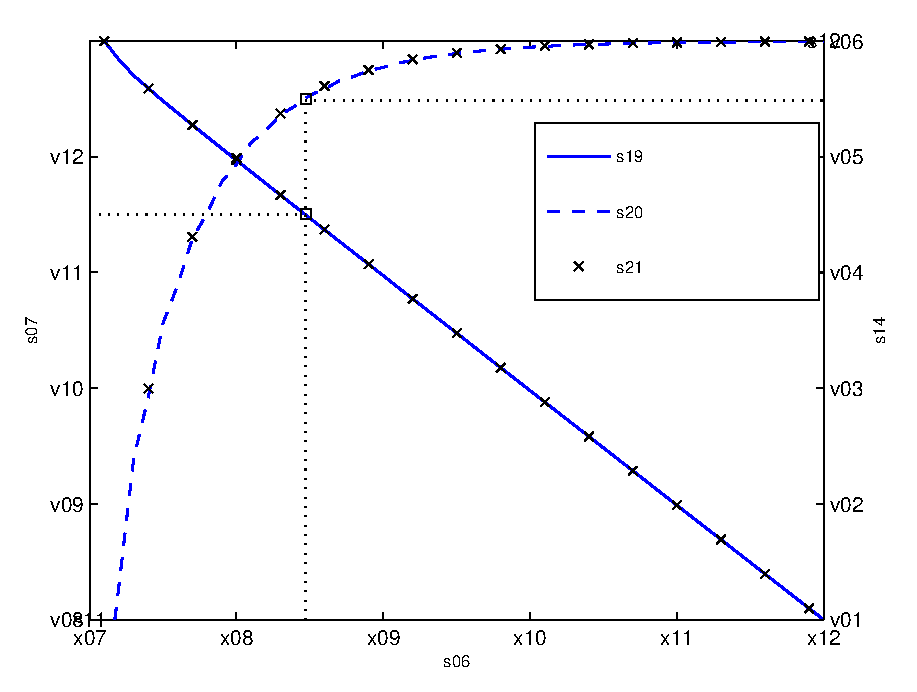
\includegraphics{ETT.eps}}%
%\end{psfrags}%
%
% End ETT.tex
\end{document}
% See http://www.mathworks.de/matlabcentral/fileexchange/loadFile.do?objectId=4638
% for recent versions of laprint.m.
%
% created by:           LaPrint version 3.16 (13.9.2004)
% created on:           23-Mar-2016 13:43:56
% eps bounding box:     16 cm x 12 cm
% comment:              
%
%\begin{psfrags}%
%\psfragscanon%
%
% text strings:
\psfrag{s06}[t][t]{\fontsize{8}{12}\fontseries{m}\mathversion{normal}\fontshape{n}\selectfont \color[rgb]{0,0,0}\setlength{\tabcolsep}{0pt}\begin{tabular}{c}$\test = [\SI{}{ms}]$\end{tabular}}%
\psfrag{s07}[b][b]{\fontsize{8}{12}\fontseries{m}\mathversion{normal}\fontshape{n}\selectfont \color[rgb]{0,0,0}\setlength{\tabcolsep}{0pt}\begin{tabular}{c}$\e{\ers}{\ers}  = [\SI{}{bits/s/Hz}]$\end{tabular}}%
\psfrag{s11}[][]{\fontsize{10}{15}\fontseries{m}\mathversion{normal}\fontshape{n}\selectfont \color[rgb]{0,0,0}\setlength{\tabcolsep}{0pt}\begin{tabular}{c} \end{tabular}}%
\psfrag{s12}[][]{\fontsize{10}{15}\fontseries{m}\mathversion{normal}\fontshape{n}\selectfont \color[rgb]{0,0,0}\setlength{\tabcolsep}{0pt}\begin{tabular}{c} \end{tabular}}%
\psfrag{s14}[t][t]{\fontsize{8}{12}\fontseries{m}\mathversion{normal}\fontshape{n}\selectfont \color[rgb]{0,0,0}\setlength{\tabcolsep}{0pt}\begin{tabular}{c}$\pco$\end{tabular}}%
\psfrag{s18}[l][l]{\fontsize{8}{12}\fontseries{m}\mathversion{normal}\fontshape{n}\selectfont \color[rgb]{0,0,0}Empirical}%
\psfrag{s19}[l][l]{\fontsize{8}{12}\fontseries{m}\mathversion{normal}\fontshape{n}\selectfont \color[rgb]{0,0,0}$\e{\ers}{\ers}$]}%
\psfrag{s20}[l][l]{\fontsize{8}{12}\fontseries{m}\mathversion{normal}\fontshape{n}\selectfont \color[rgb]{0,0,0}$\pco$}%
\psfrag{s21}[l][l]{\fontsize{8}{12}\fontseries{m}\mathversion{normal}\fontshape{n}\selectfont \color[rgb]{0,0,0}Empirical}%
%
% axes font properties:
\fontsize{8}{12}\fontseries{m}\mathversion{normal}%
\fontshape{n}\selectfont%
%
% xticklabels:
\psfrag{x01}[t][t]{0}%
\psfrag{x02}[t][t]{0.5}%
\psfrag{x03}[t][t]{1}%
\psfrag{x04}[t][t]{1.5}%
\psfrag{x05}[t][t]{2}%
\psfrag{x06}[t][t]{2.5}%
\psfrag{x07}[t][t]{0}%
\psfrag{x08}[t][t]{0.5}%
\psfrag{x09}[t][t]{1}%
\psfrag{x10}[t][t]{1.5}%
\psfrag{x11}[t][t]{2}%
\psfrag{x12}[t][t]{2.5}%
%
% yticklabels:
\psfrag{v01}[l][l]{0.50}%
\psfrag{v02}[l][l]{0.60}%
\psfrag{v03}[l][l]{0.70}%
\psfrag{v04}[l][l]{0.80}%
\psfrag{v05}[l][l]{0.90}%
\psfrag{v06}[l][l]{1.00}%
\psfrag{v07}[l][l]{}%
\psfrag{v08}[r][r]{6.89}%
\psfrag{v09}[r][r]{6.93}%
\psfrag{v10}[r][r]{6.96}%
\psfrag{v11}[r][r]{7.00}%
\psfrag{v12}[r][r]{7.04}%
\psfrag{v13}[r][r]{7.07}%
\psfrag{v14}[r][r]{}%
%
% Figure:
%\resizebox{8cm}{!}{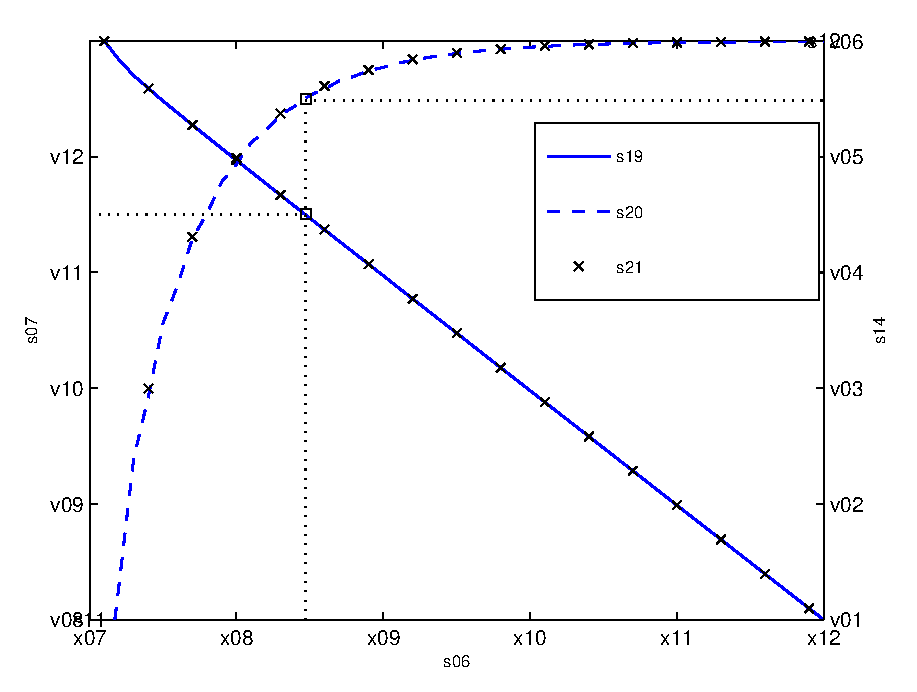
\includegraphics{ETT.eps}}%
%\end{psfrags}%
%
% End ETT.tex
\end{document}
% See http://www.mathworks.de/matlabcentral/fileexchange/loadFile.do?objectId=4638
% for recent versions of laprint.m.
%
% created by:           LaPrint version 3.16 (13.9.2004)
% created on:           01-Apr-2016 10:19:15
% eps bounding box:     16 cm x 12 cm
% comment:              
%
%\begin{psfrags}%
%\psfragscanon%
%
% text strings:
\psfrag{s06}[t][t]{\fontsize{8}{12}\fontseries{m}\mathversion{normal}\fontshape{n}\selectfont \color[rgb]{0,0,0}\setlength{\tabcolsep}{0pt}\begin{tabular}{c}$\test$ [\SI{}{ms}]\end{tabular}}%
\psfrag{s07}[b][b]{\fontsize{8}{12}\fontseries{m}\mathversion{normal}\fontshape{n}\selectfont \color[rgb]{0,0,0}\setlength{\tabcolsep}{0pt}\begin{tabular}{c}$\rs$ [\SI{}{bits/s/Hz}]\end{tabular}}%
\psfrag{s11}[][]{\fontsize{10}{15}\fontseries{m}\mathversion{normal}\fontshape{n}\selectfont \color[rgb]{0,0,0}\setlength{\tabcolsep}{0pt}\begin{tabular}{c} \end{tabular}}%
\psfrag{s12}[][]{\fontsize{10}{15}\fontseries{m}\mathversion{normal}\fontshape{n}\selectfont \color[rgb]{0,0,0}\setlength{\tabcolsep}{0pt}\begin{tabular}{c} \end{tabular}}%
\psfrag{s14}[t][t]{\fontsize{8}{12}\fontseries{m}\mathversion{normal}\fontshape{n}\selectfont \color[rgb]{0,0,0}\setlength{\tabcolsep}{0pt}\begin{tabular}{c}$\pco$\end{tabular}}%
\psfrag{s18}[l][l]{\fontsize{8}{12}\fontseries{m}\mathversion{normal}\fontshape{n}\selectfont \color[rgb]{0,0,0}Empirical}%
\psfrag{s19}[l][l]{\fontsize{8}{12}\fontseries{m}\mathversion{normal}\fontshape{n}\selectfont \color[rgb]{0,0,0}$\rs$}%
\psfrag{s20}[l][l]{\fontsize{8}{12}\fontseries{m}\mathversion{normal}\fontshape{n}\selectfont \color[rgb]{0,0,0}$\pco$}%
\psfrag{s21}[l][l]{\fontsize{8}{12}\fontseries{m}\mathversion{normal}\fontshape{n}\selectfont \color[rgb]{0,0,0}Empirical}%
%
% axes font properties:
\fontsize{8}{12}\fontseries{m}\mathversion{normal}%
\fontshape{n}\selectfont%
%
% xticklabels:
\psfrag{x01}[t][t]{0}%
\psfrag{x02}[t][t]{0.5}%
\psfrag{x03}[t][t]{1}%
\psfrag{x04}[t][t]{1.5}%
\psfrag{x05}[t][t]{2}%
\psfrag{x06}[t][t]{2.5}%
\psfrag{x07}[t][t]{0}%
\psfrag{x08}[t][t]{0.5}%
\psfrag{x09}[t][t]{1}%
\psfrag{x10}[t][t]{1.5}%
\psfrag{x11}[t][t]{2}%
\psfrag{x12}[t][t]{2.5}%
%
% yticklabels:
\psfrag{v01}[l][l]{0.50}%
\psfrag{v02}[l][l]{0.60}%
\psfrag{v03}[l][l]{0.70}%
\psfrag{v04}[l][l]{0.80}%
\psfrag{v05}[l][l]{0.90}%
\psfrag{v06}[l][l]{1.00}%
\psfrag{v07}[l][l]{}%
\psfrag{v08}[r][r]{6.89}%
\psfrag{v09}[r][r]{6.93}%
\psfrag{v10}[r][r]{6.96}%
\psfrag{v11}[r][r]{7.00}%
\psfrag{v12}[r][r]{7.04}%
\psfrag{v13}[r][r]{7.07}%
\psfrag{v14}[r][r]{}%
%
% Figure:
%\resizebox{8cm}{!}{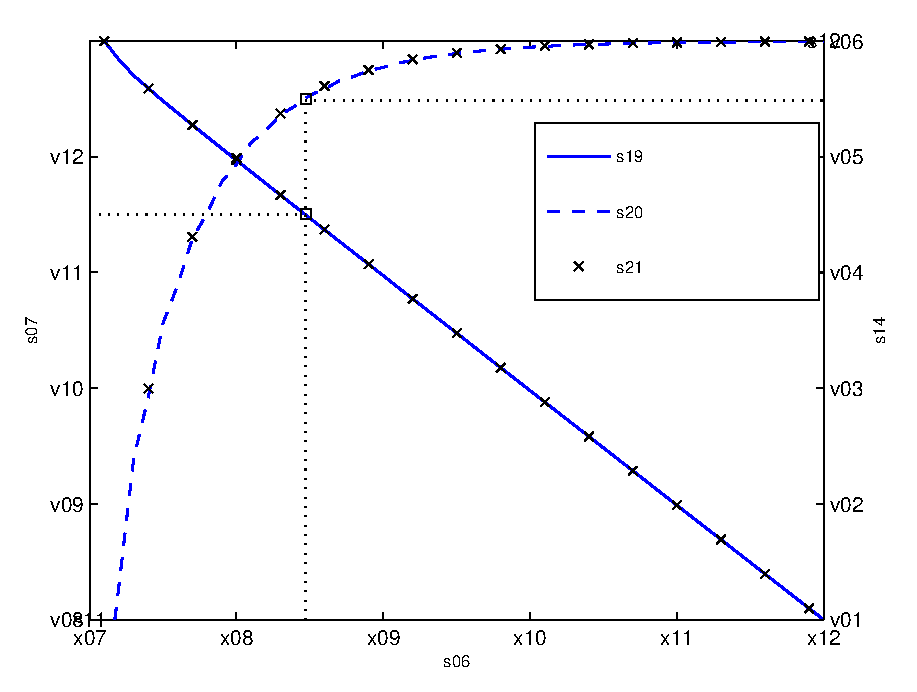
\includegraphics{ETT.eps}}%
%\end{psfrags}%
%
% End ETT.tex
